\documentclass{standalone}
\usepackage{tikz}
\usetikzlibrary{patterns, positioning}

\begin{document}
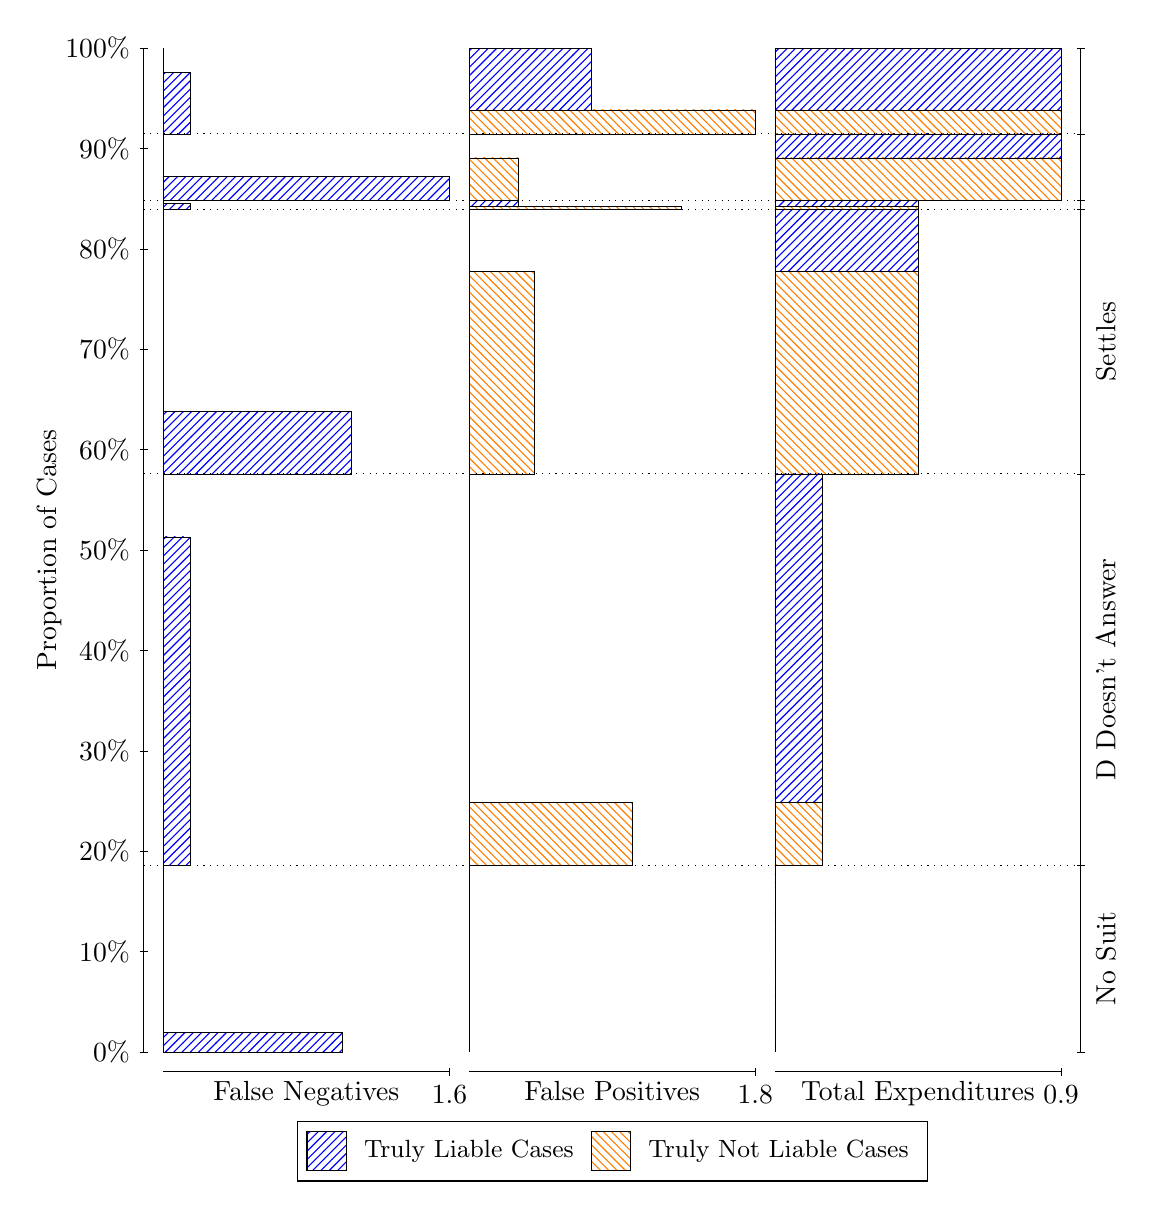
\begin{tikzpicture}
\draw[black, very thin] (1.5,1.75) -- (1.5,14.5);
\node[rotate=90, anchor=center] at (0.3, 8.125) {Proportion of Cases};
\draw[black, very thin] (1.45,1.75) -- (1.55,1.75);
\node[anchor=east] at (1.45, 1.75) {0\%};
\draw[black, very thin] (1.45,3.025) -- (1.55,3.025);
\node[anchor=east] at (1.45, 3.025) {10\%};
\draw[black, very thin] (1.45,4.3) -- (1.55,4.3);
\node[anchor=east] at (1.45, 4.3) {20\%};
\draw[black, very thin] (1.45,5.575) -- (1.55,5.575);
\node[anchor=east] at (1.45, 5.575) {30\%};
\draw[black, very thin] (1.45,6.85) -- (1.55,6.85);
\node[anchor=east] at (1.45, 6.85) {40\%};
\draw[black, very thin] (1.45,8.125) -- (1.55,8.125);
\node[anchor=east] at (1.45, 8.125) {50\%};
\draw[black, very thin] (1.45,9.4) -- (1.55,9.4);
\node[anchor=east] at (1.45, 9.4) {60\%};
\draw[black, very thin] (1.45,10.675) -- (1.55,10.675);
\node[anchor=east] at (1.45, 10.675) {70\%};
\draw[black, very thin] (1.45,11.95) -- (1.55,11.95);
\node[anchor=east] at (1.45, 11.95) {80\%};
\draw[black, very thin] (1.45,13.225) -- (1.55,13.225);
\node[anchor=east] at (1.45, 13.225) {90\%};
\draw[black, very thin] (1.45,14.5) -- (1.55,14.5);
\node[anchor=east] at (1.45, 14.5) {100\%};

\draw[black, very thin] (13.4,1.75) -- (13.4,14.5);
\draw[black, very thin] (13.35,1.75) -- (13.45,1.75);
\node[anchor=west] at (13.35, 1.75) {};
\draw[black, very thin] (13.35,4.1224) -- (13.45,4.1224);
\node[anchor=west] at (13.35, 4.1224) {};
\draw[black, very thin] (13.35,9.0921) -- (13.45,9.0921);
\node[anchor=west] at (13.35, 9.0921) {};
\draw[black, very thin] (13.35,12.451) -- (13.45,12.451);
\node[anchor=west] at (13.35, 12.451) {};
\draw[black, very thin] (13.35,12.562) -- (13.45,12.562);
\node[anchor=west] at (13.35, 12.562) {};
\draw[black, very thin] (13.35,13.41) -- (13.45,13.41);
\node[anchor=west] at (13.35, 13.41) {};
\draw[black, very thin] (13.35,14.5) -- (13.45,14.5);
\node[anchor=west] at (13.35, 14.5) {};

\draw[black, very thin, pattern color=blue, pattern=north east lines] (1.75,1.75) rectangle (4.0208,1.9996);
\draw[black, very thin, pattern color=orange, pattern=north west lines] (1.75,1.9996) rectangle (1.75,4.1224);
\draw[black, very thin, pattern color=blue, pattern=north east lines] (1.75,4.1224) rectangle (2.0906,8.2905);
\draw[black, very thin, pattern color=orange, pattern=north west lines] (1.75,8.2905) rectangle (1.75,9.0921);
\draw[black, very thin, pattern color=blue, pattern=north east lines] (1.75,9.0921) rectangle (4.1344,9.8831);
\draw[black, very thin, pattern color=orange, pattern=north west lines] (1.75,9.8831) rectangle (1.75,12.451);
\draw[black, very thin, pattern color=blue, pattern=north east lines] (1.75,12.451) rectangle (2.0906,12.528);
\draw[black, very thin, pattern color=orange, pattern=north west lines] (1.75,12.528) rectangle (1.75,12.562);
\draw[black, very thin, pattern color=blue, pattern=north east lines] (1.75,12.562) rectangle (5.3833,12.866);
\draw[black, very thin, pattern color=orange, pattern=north west lines] (1.75,12.866) rectangle (1.75,13.41);
\draw[black, very thin, pattern color=blue, pattern=north east lines] (1.75,13.41) rectangle (2.0906,14.195);
\draw[black, very thin, pattern color=orange, pattern=north west lines] (1.75,14.195) rectangle (1.75,14.5);
\draw[black, very thin, pattern color=orange, pattern=north west lines] (5.6333,1.75) rectangle (5.6333,3.8728);
\draw[black, very thin, pattern color=blue, pattern=north east lines] (5.6333,3.8728) rectangle (5.6333,4.1224);
\draw[black, very thin, pattern color=orange, pattern=north west lines] (5.6333,4.1224) rectangle (7.7095,4.924);
\draw[black, very thin, pattern color=blue, pattern=north east lines] (5.6333,4.924) rectangle (5.6333,9.0921);
\draw[black, very thin, pattern color=orange, pattern=north west lines] (5.6333,9.0921) rectangle (6.4638,11.66);
\draw[black, very thin, pattern color=blue, pattern=north east lines] (5.6333,11.66) rectangle (5.6333,12.451);
\draw[black, very thin, pattern color=orange, pattern=north west lines] (5.6333,12.451) rectangle (8.3324,12.486);
\draw[black, very thin, pattern color=blue, pattern=north east lines] (5.6333,12.486) rectangle (6.2562,12.562);
\draw[black, very thin, pattern color=orange, pattern=north west lines] (5.6333,12.562) rectangle (6.2562,13.105);
\draw[black, very thin, pattern color=blue, pattern=north east lines] (5.6333,13.105) rectangle (5.6333,13.41);
\draw[black, very thin, pattern color=orange, pattern=north west lines] (5.6333,13.41) rectangle (9.2667,13.714);
\draw[black, very thin, pattern color=blue, pattern=north east lines] (5.6333,13.714) rectangle (7.1905,14.5);
\draw[black, very thin, pattern color=orange, pattern=north west lines] (9.5167,1.75) rectangle (9.5167,3.8728);
\draw[black, very thin, pattern color=blue, pattern=north east lines] (9.5167,3.8728) rectangle (9.5167,4.1224);
\draw[black, very thin, pattern color=orange, pattern=north west lines] (9.5167,4.1224) rectangle (10.122,4.924);
\draw[black, very thin, pattern color=blue, pattern=north east lines] (9.5167,4.924) rectangle (10.122,9.0921);
\draw[black, very thin, pattern color=orange, pattern=north west lines] (9.5167,9.0921) rectangle (11.333,11.66);
\draw[black, very thin, pattern color=blue, pattern=north east lines] (9.5167,11.66) rectangle (11.333,12.451);
\draw[black, very thin, pattern color=orange, pattern=north west lines] (9.5167,12.451) rectangle (11.333,12.486);
\draw[black, very thin, pattern color=blue, pattern=north east lines] (9.5167,12.486) rectangle (11.333,12.562);
\draw[black, very thin, pattern color=orange, pattern=north west lines] (9.5167,12.562) rectangle (13.15,13.105);
\draw[black, very thin, pattern color=blue, pattern=north east lines] (9.5167,13.105) rectangle (13.15,13.41);
\draw[black, very thin, pattern color=orange, pattern=north west lines] (9.5167,13.41) rectangle (13.15,13.714);
\draw[black, very thin, pattern color=blue, pattern=north east lines] (9.5167,13.714) rectangle (13.15,14.5);
\draw[black, dotted] (1.5,4.1224) -- (13.4,4.1224);
\draw[black, dotted] (1.5,9.0921) -- (13.4,9.0921);
\draw[black, dotted] (1.5,12.451) -- (13.4,12.451);
\draw[black, dotted] (1.5,12.562) -- (13.4,12.562);
\draw[black, dotted] (1.5,13.41) -- (13.4,13.41);
\draw[black, very thin] (1.75,1.5) -- (5.3833,1.5);
\node[anchor=north] at (3.5667, 1.5) {False Negatives};
\draw[black, very thin] (5.3833,1.45) -- (5.3833,1.55);
\node[anchor=north] at (5.3833, 1.45) {1.6};

\draw[black, very thin] (5.6333,1.5) -- (9.2667,1.5);
\node[anchor=north] at (7.45, 1.5) {False Positives};
\draw[black, very thin] (9.2667,1.45) -- (9.2667,1.55);
\node[anchor=north] at (9.2667, 1.45) {1.8};

\draw[black, very thin] (9.5167,1.5) -- (13.15,1.5);
\node[anchor=north] at (11.333, 1.5) {Total Expenditures};
\draw[black, very thin] (13.15,1.45) -- (13.15,1.55);
\node[anchor=north] at (13.15, 1.45) {0.9};

\node[black, centered, rotate=90] at (13.72, 2.9362) {No Suit};
\node[black, centered, rotate=90] at (13.72, 6.6072) {D Doesn't Answer};
\node[black, centered, rotate=90] at (13.72, 10.772) {Settles};




\draw (7.449999999999999,1.5) node[draw=none] (baseCoordinate) {};
\begin{scope}[align=center]
        \matrix[scale=0.5, draw=black, below=0.5cm of baseCoordinate, nodes={draw}, column sep=0.1cm]{
            \node[rectangle, draw, minimum width=0.5cm, minimum height=0.5cm, pattern=north east lines, pattern color=blue] {}; &
            \node[draw=none, font=\small] (B) {Truly Liable Cases}; &
            \node[rectangle, draw, minimum width=0.5cm, minimum height=0.5cm, pattern=north west lines, pattern color=orange] {}; &
            \node[draw=none, font=\small] (B) {Truly Not Liable Cases}; \\
            };
\end{scope}

\end{tikzpicture}
\end{document}